\documentclass[tikz]{standalone}
\renewcommand*{\familydefault}{\sfdefault}
\usepackage{standalone}
\usepackage{amssymb}
\usetikzlibrary{decorations}
%\usetikzlibrary{arrows.meta, decorations.pathmorphing, decorations.pathreplacing, shapes.geometric}
\usetikzlibrary{bayesnet}

\begin{document}
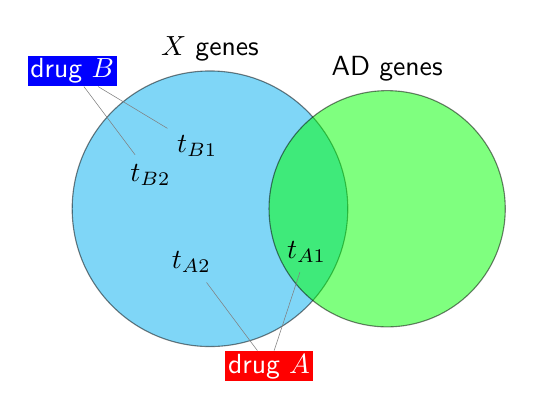
\begin{tikzpicture}[pin distance=1.0cm]%[font=\footnotesize, xscale=1.5]
\draw[draw,fill=cyan,semitransparent] (0.25,0) circle(1.75);
\draw[draw,fill=green,semitransparent] (2.5,0) circle(1.5);
%\draw (0,0) circle(3) (4,0) circle(4);
\path (1,-2) node[white,rectangle,inner sep=1pt,fill=red,
	pin=85:$t_{A1}$,
	pin=120:$t_{A2}$] {drug $A$};
\path (-1.5,1.75) node[white,rectangle,inner sep=1pt,fill=blue,
	pin=-30:$t_{B1}$,
	pin=-60:$t_{B2}$] {drug $B$};
\node[anchor=south] (X) at (0.25,1.75) {$X$ genes};
\node[anchor=south] (X) at (2.5,1.5) {AD genes};
\end{tikzpicture}
\end{document}
